% Setup - do not change
\documentclass[11pt]{article}
\usepackage[top=0.9in, left=0.9in, bottom=0.9in, right=0.9in]{geometry} 
\usepackage{parskip}

\usepackage[english]{babel}
\usepackage[utf8]{inputenc}
\usepackage{amsmath,amsthm,amssymb,graphicx,pdfpages,lipsum,hyperref}
\usepackage[none]{hyphenat}
\usepackage{csquotes}

\usepackage{graphicx}
\usepackage{subcaption}
\usepackage{mwe}
\usepackage{float}
\usepackage{tabularx}

\setlength\parindent{0pt}
%%%%%%%%%%%%%%%%%%%%%%%%%%%%%%%%%%%%%%%%%%%%%%%%%%%%%%%%%%%%%%%%%%%
% add other packages here if required

%% Bibliography are specified in this file. You can also choose inline bib style if you want to. But make sure your citation style is consistent (and proper)
% For more details on citation: https://library.unimelb.edu.au/recite
\usepackage[sorting = none]{biblatex}
\addbibresource{references.bib}

%%%%%%%%%%%%%%%%%%%%%%%%%%%%%%%%%%%%%%%%%%%%%%%%%%%%%%%%%%%%%%%%%%% the '%' symbol denotes comments

% Begin document creation
% DELETE THE \lipsum PLACEHOLDERS WHEN YOU BEGIN
\author{
Kelman Chen \\ 
Student ID: 1168867 \\
%% Replace the link with your github repo
% 1. Remember to escape underscore (\_) in the link.
% 2. Remember to include the commit you want to submit in the link
\href{https://github.com/MAST30034-Applied-Data-Science/mast30034-project-1-kelmanchen.git}{Github repo with commit}
}

\begin{document}
\maketitle

\section{Introduction}
% Link to a 30 min tutorial if you require revision: https://www.overleaf.com/learn/latex/Learn_LaTeX_in_30_minutes

In early 2021, New York City (NYC) began reopening following the outbreak of the COVID-19 pandemic as vaccines were introduced \cite{NYC_covid_timeline}.  Unfortunately, the pandemic was far from over as the entire nation saw a huge spike in both case numbers and deaths in the middle of the holiday season from December 2021 to February 2022. Amongst all this, one of the industries that was hit the hardest was NYC's Taxi and ``High Volume'' ride-share services.

This report will aim to explore the impact of the late 2021 spike on the Yellow Taxi and High Volume For-Hire Vehicles (HVFHV) industry, and how passenger behaviour and trends may have changed during the holiday season following all the lock-downs that NYC faced. 

Throughout this report, data will be analysed through geospatial information, analysis of relationships between features and comparisons of various timelines before modelling passenger behaviour through Linear Regression. Recommendations will then be made to key decision makers of both Yellow Taxi and HVFHV companies through the results of the analysis and modelling.

\section{Data-set}

The report primarily makes use of data published by the Taxi \& Limousine Commission (NYC TLC) \cite{TLC_data}. The data-sets chosen were the Yellow Taxi and HVFHV records for the period December 2019 to February 2020, and December 2021 to February 2022. The decision to use these periods is to allow for comparison between just before the pandemic (2019-2020), and the largest spike in case numbers in NYC (2021-2022) while limiting external factors such as seasonal weather and holiday periods. Additionally, COVID-19 daily case numbers and hospitalisations are used in relation to the December 2021 to February 2022 period. 

Throughout this report, December 2019 to February 2020 will be abbreviated to 2019-2020, and December 2021 to February 2022 to 2021-2022. 

\subsection{Yellow Taxi Data}
The Yellow Taxi data-set was chosen as they are the only vehicles permitted to respond to a street hail from a passenger in all five
boroughs.

The attributes investigated include total fare amounts; tip amounts as a percentage of fare amounts; trip time and distance; and pickup and drop-off locations and dates as these will give the best indication of passenger behaviours. From these, the number of trips were aggregated by date. 

\subsection{HVFHV Data}
The HVFHV industry such as Uber and Lyft have dominated NYC's taxi industry. This data-set was chosen to examine its recovery rate compared to that of Yellow Taxis. 

Attributes investigated in this data-set are the same as Yellow Taxi to allow for the easiest comparison.

\subsection{COVID-19 Data}
To accurately investigate the effects of COVID-19, data was sourced from the NYC Open Data site \cite{COVID_data}.

Both daily case numbers of interest and daily hospitalisations are included to analyse whether one certain feature is particularly correlated with that of the TLC data-sets. 

\section{Pre-processing}
As with all large data-sets, a reasonable amount of pre-processing was required to ensure the data was well suited for analysis. This section outlines feature engineering, outlier detection and cleansing, and selection of relevant features. 

\subsection{Feature Engineering}
Feature engineering is necessary in these data-sets as not all useful features are present but can be derived.

\begin{itemize}
    \item For the Yellow Taxi data-set, \textbf{trip duration} in minutes was calculated using the difference between pickup and drop-off times
    \item For the HVFHV data-set, the \textbf{total amount} was calculated using the base passenger fare, tolls, sales tax, tips and airport fee
    \item For both Yellow Taxi and HVFHV data-sets, the \textbf{tip percentage} was calculated using the tip and total amounts
\end{itemize}

Furthermore, the format of the data-sets such as feature names were not always consistent with each other, therefore features were renamed accordingly and trip duration for HVFHV was converted to minutes. 

\subsection{Cleaning}
This section outlines the criteria for cleaning of the data-sets. Upon using a box-plot to detect outliers, various records were removed based on examining these plots and using rules of each attribute in  reality. These box-plot visualisation were generated only using 5\% of the 2019-2020 Yellow Taxi data-set and were thus only used as a guide. 

\subsubsection{NYC TLC Data}
The following steps were taken to clean both the Yellow Taxi and HVFHV data-sets:
\begin{itemize}
    \item \textbf{Removed records where trip time was less than 0 minutes or more than 300 minutes.} The upper limit was determined by taking the time of the 4th longest Uber Ride (approximately 5 hours) \cite{longest_ubers}, as anything longer may have been incorrectly entered or irrelevant for analysis
    \item \textbf{Removed records where the total fare amount was less than \$0 and more than \$400.} The upper limit was determined by overview of the box-plot and the approximate cost of the 4th longest Uber Ride \cite{longest_ubers} 
    \item \textbf{Removed records with passenger counts not between 1 and 6.} The maximum allowed passengers including children in Yellow Taxis is 6 \cite{YT_max_passengers} (Yellow Taxis data-set only)
    \item \textbf{Removed records with trip distance less than 0 miles and more than 300 miles.} The upper limit was determined by overview of the box-plot and the approximate distance of the 4th longest Uber Ride \cite{longest_ubers}
    \item \textbf{Removed records where the tip amount was less than \$0 or more than the total amount}
    \item \textbf{Filtered records only with payment type 1.} Only credit card payments were considered as tips were not tracked for cash payments. (Yellow Taxis data-set only)
    \item \textbf{Removed records with invalid pickup and drop-off location IDs.} Location IDs must be between 1 and 263
\end{itemize}

Approximately 8 million records in total were removed from the Yellow Taxi data-sets, and 1.5 million removed from the HVFHV data-sets following data cleaning. 

\subsubsection{COVID-19 Data}
For the COVID-19 data-set the only cleaning and standardisation required was to convert the date of interest features to the same date-time format as the NYC TLC Data. Otherwise, the data-set was of high quality and usable with minimal processing.

\section{Visualisation and Analysis}
To explore the effects of COVID-19 on the industry, this section will investigate relationships between various features as well as changes of features over time. 

\subsection{Geospatial Analysis}
A large impact as a result of COVID-19 was international travel. Considering a large proportion of the model of travel to/from airports are via Taxi and HVFHV services, John F. Kennedy (JFK) Airport - the busiest international airport in NYC - is explored \cite{JFK_airport}.

For these visualisations, a 5\% random sample of the data was used.

\subsubsection{Pickup Counts}

As shown in Figure 1, it is fairly clear that many of the trips by both Yellow Taxis and HVFHV are concentrated especially at JFK Airport. In the Yellow Taxis, there seems to be a slight increase in proportion of trips beginning in JFK airport as seen in Figures 1a and 1b, whereas a change in proportion is less evident in HVFHV as observed in Figures 1c and 1d. 

\begin{figure*}
    \centering
    \begin{subfigure}[b]{0.4\textwidth}
        \centering
        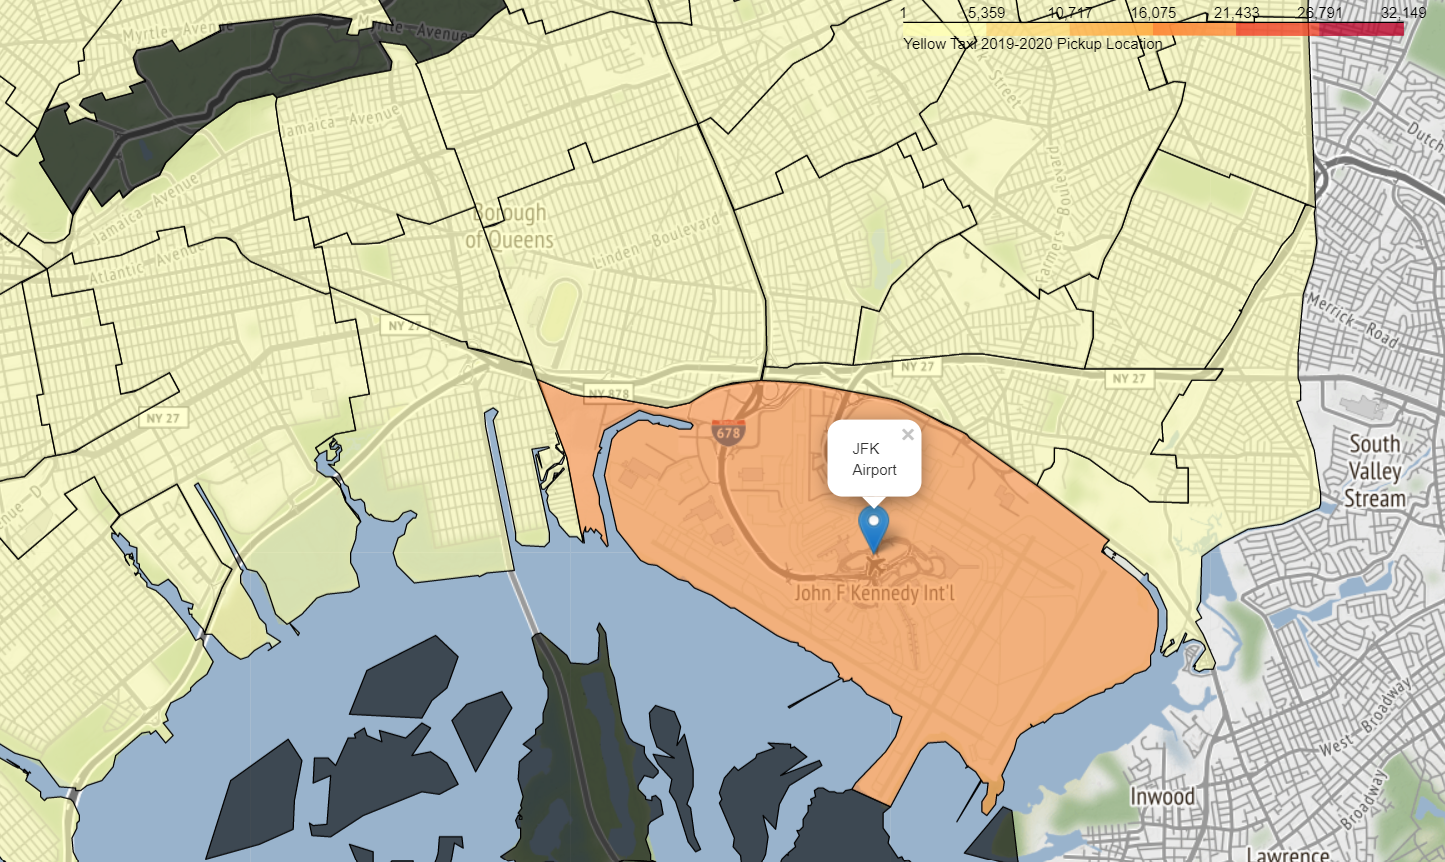
\includegraphics[width=\textwidth]{plots/yellow_19_20_PULoc_geomap.png}
        \caption[]%
        {{\small Yellow Taxi 2019-2020}}    
        \label{}
    \end{subfigure}
    \hfill
    \begin{subfigure}[b]{0.4\textwidth}  
        \centering 
        \includegraphics[width=\textwidth]{plots/yellow_21_22_PULoc_geomap.png}
        \caption[]%
        {{\small Yellow Taxi 2021-2022}}    
        \label{}
    \end{subfigure}
    \vskip\baselineskip
    \begin{subfigure}[b]{0.4\textwidth}   
        \centering 
        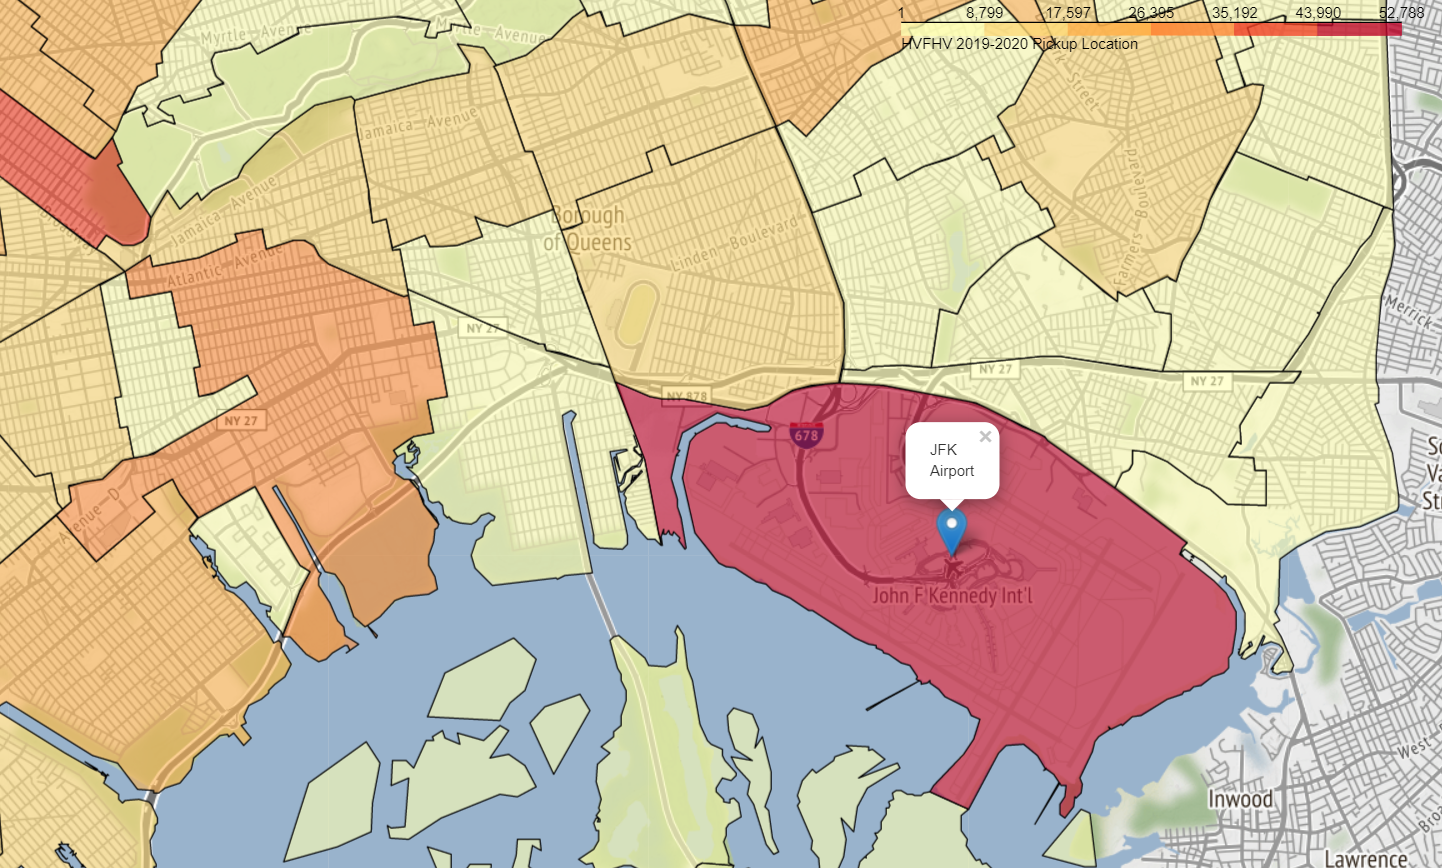
\includegraphics[width=\textwidth]{plots/hvfhv_19_20_PULoc_geomap.png}
        \caption[]%
        {{\small HVFHV 2019-2020}}    
        \label{}
    \end{subfigure}
    \hfill
    \begin{subfigure}[b]{0.4\textwidth}   
        \centering 
        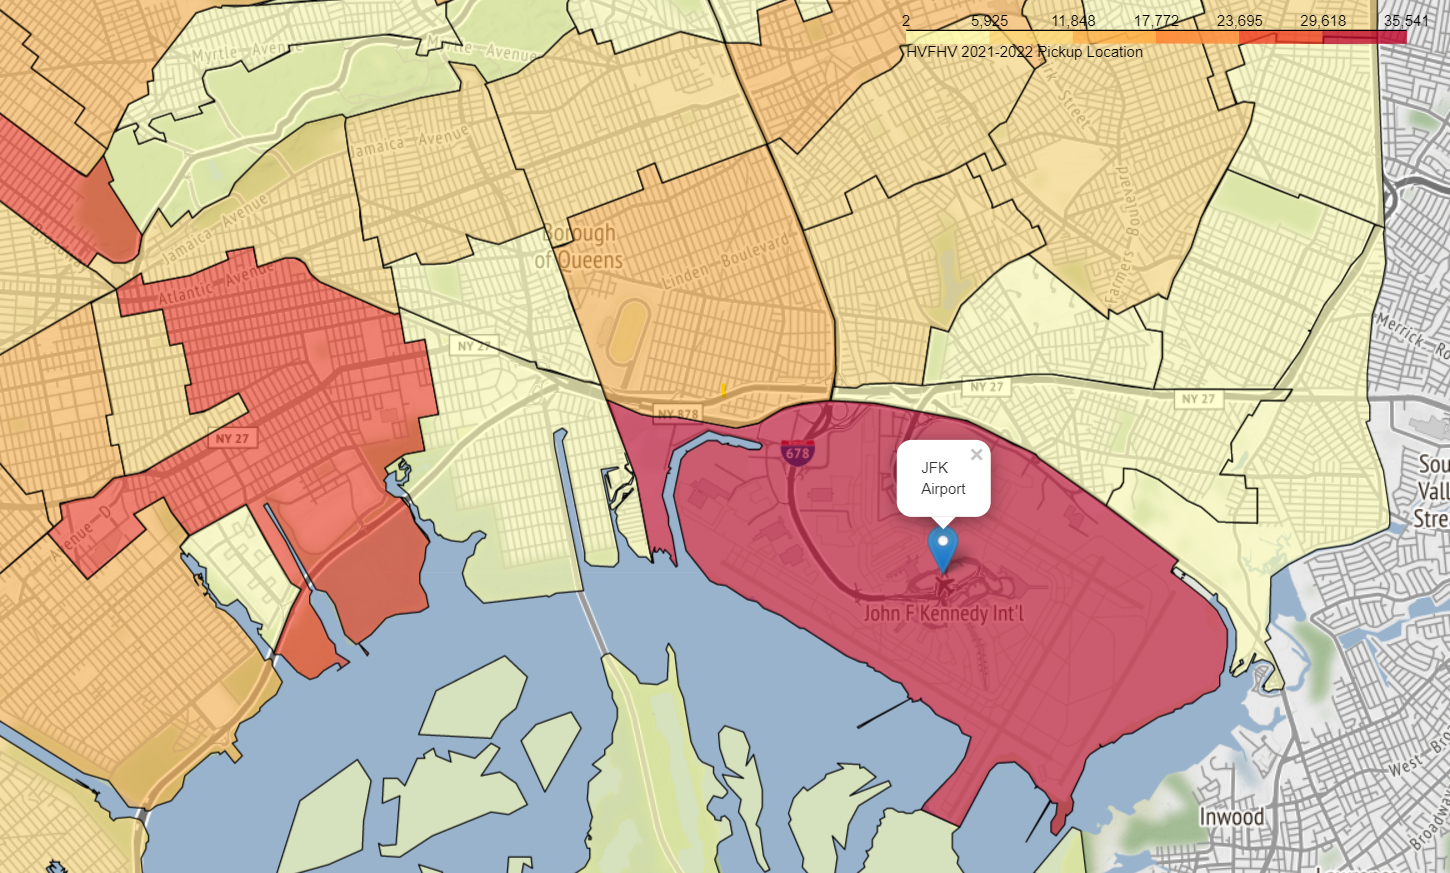
\includegraphics[width=\textwidth]{plots/hvfhv_21_22_PULoc_geomap.png}
        \caption[]%
        {{\small HVFHV 2021-2022}}    
        \label{}
    \end{subfigure}
    \caption[]
    {\small Total pickup counts by Taxi Zone} 
    \label{}
\end{figure*}

\subsubsection{Drop-off Counts}

\begin{figure*}
    \centering
    \begin{subfigure}[b]{0.4\textwidth}
        \centering
        \includegraphics[width=\textwidth]{plots/yellow_19_20_DOLoc_geomap.png}
        \caption[]%
        {{\small Yellow Taxi 2019-2020}}    
        \label{}
    \end{subfigure}
    \hfill
    \begin{subfigure}[b]{0.4\textwidth}  
        \centering 
        \includegraphics[width=\textwidth]{plots/yellow_21_22_DOLoc_geomap.png}
        \caption[]%
        {{\small Yellow Taxi 2021-2022}}    
        \label{}
    \end{subfigure}
    \vskip\baselineskip
    \begin{subfigure}[b]{0.4\textwidth}   
        \centering 
        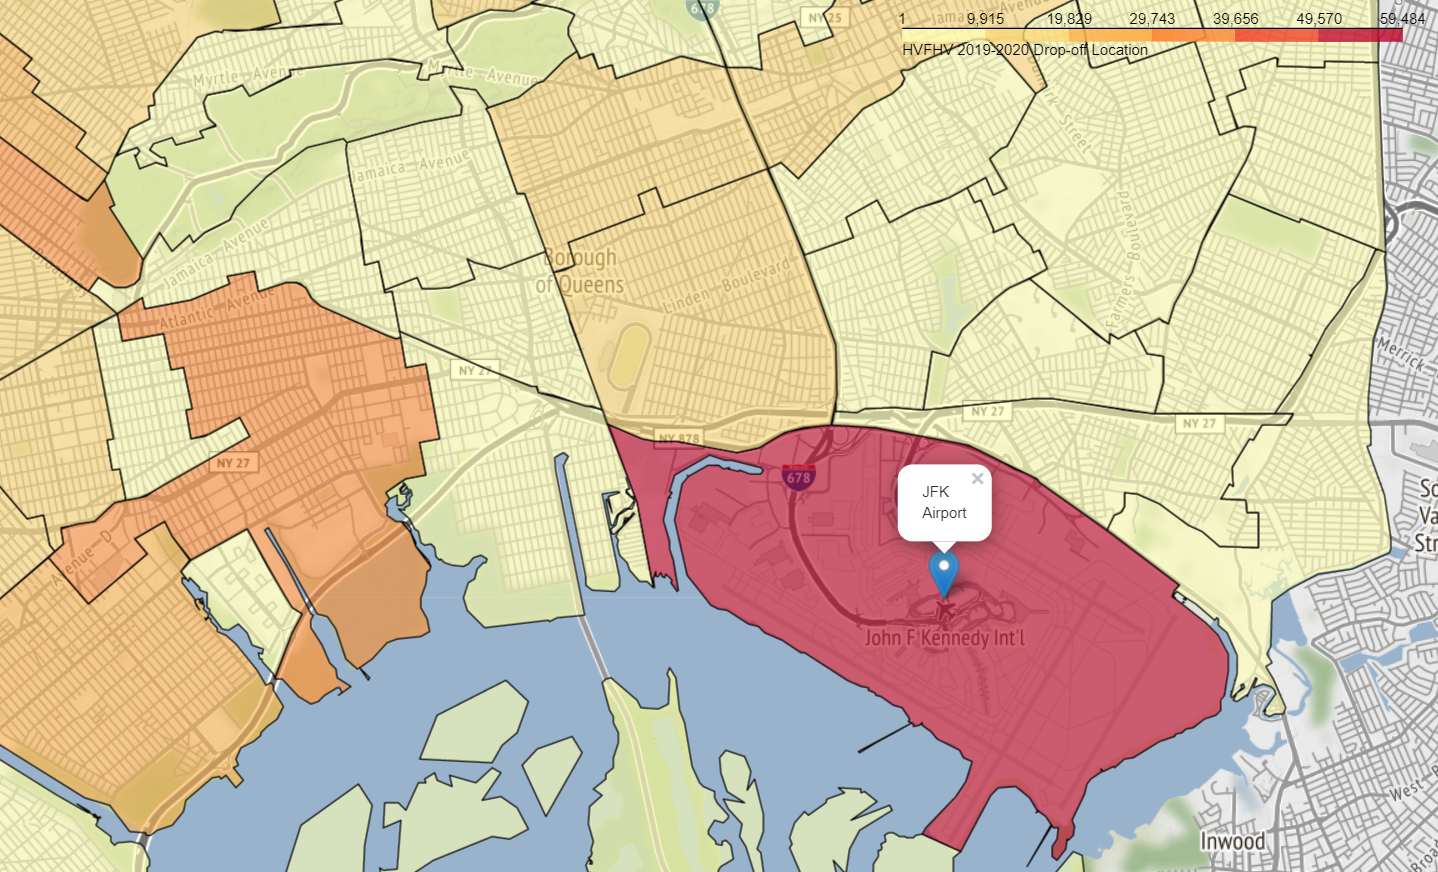
\includegraphics[width=\textwidth]{plots/hvfhv_19_20_DOLoc_geomap.png}
        \caption[]%
        {{\small HVFHV 2019-2020}}    
        \label{}
    \end{subfigure}
    \hfill
    \begin{subfigure}[b]{0.4\textwidth}   
        \centering 
        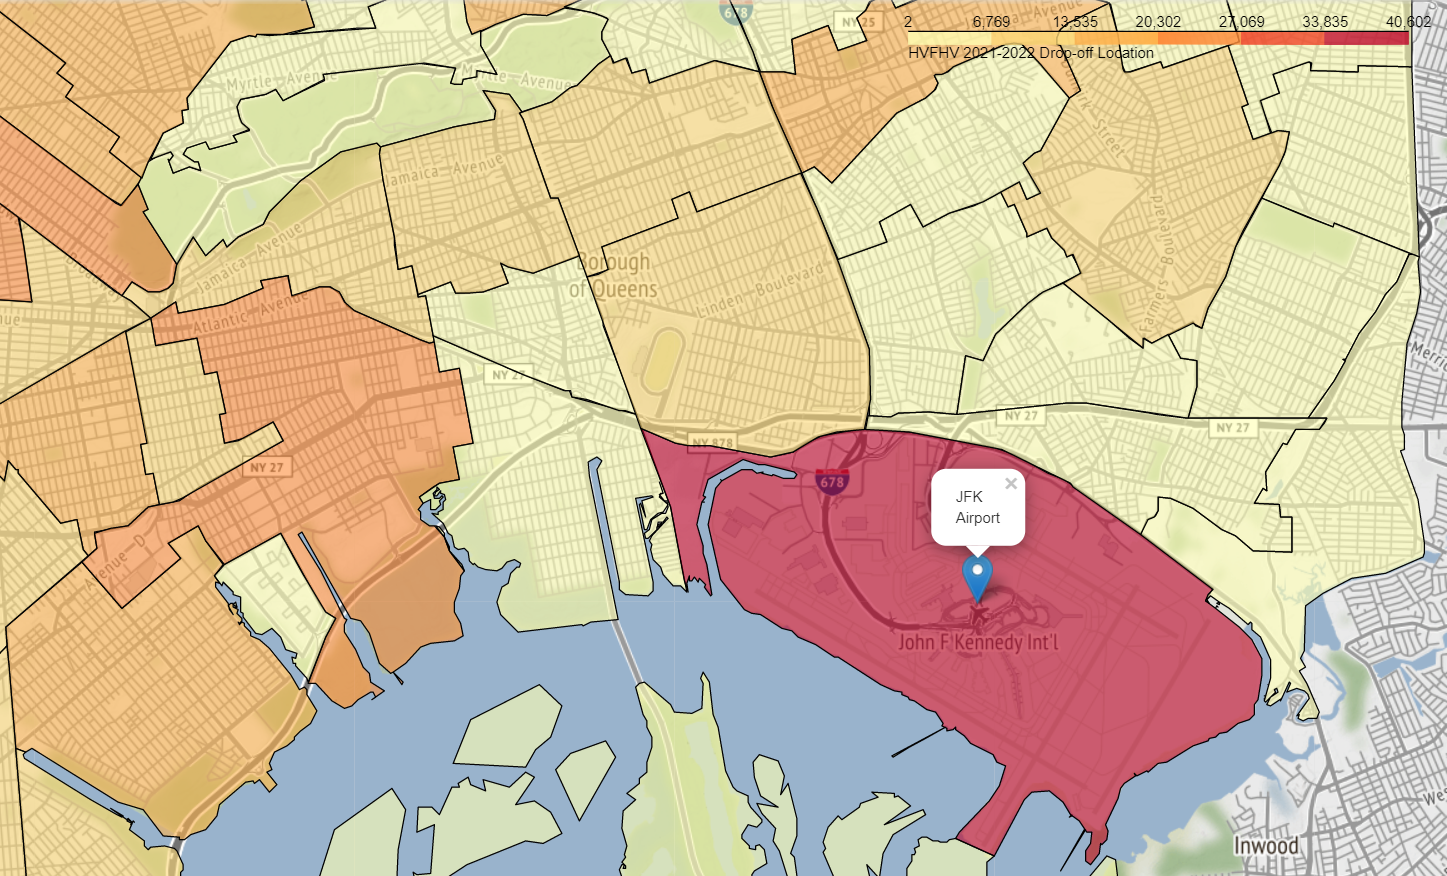
\includegraphics[width=\textwidth]{plots/hvfhv_21_22_DOLoc_geomap.png}
        \caption[]%
        {{\small HVFHV 2021-2022}}    
        \label{}
    \end{subfigure}
    \caption[]
    {\small Total drop-off counts by Taxi Zone} 
    \label{}
\end{figure*}

Interestingly, Yellow Taxis as can been seen in Figures 2a and 2b seem to have a fairly small proportion when it comes to drop-offs to JFK Airport compared to HVFHV. While the HVFHV maps in Figures 2c and 2d don't have noticeable changes in proportions of drop-offs to JFK Airport, the Yellow Taxis have a slight decrease in 2021-2022 compared to 2019-2020.

While there are slight changes of proportions in Yellow Taxis and lack of change in HVFHV of both pickup and drop-off trip counts, the legend in all the sub-figures of both Figure 1 and Figure 2 indicate a decline in trip counts in 2021-2022 compared to 2019-2020 and shows the effects of COVID-19 on travel in all locations.


\subsection{Feature Relationships Analysis}
In this section, we investigate relationships between features in order to explore possible correlation between features and how COVID-19 has affected the industry. The Yellow Taxi and HVFHV data-sets were aggregated by date to allow for correlation comparisons.

\begin{figure}[H]
    \centering
    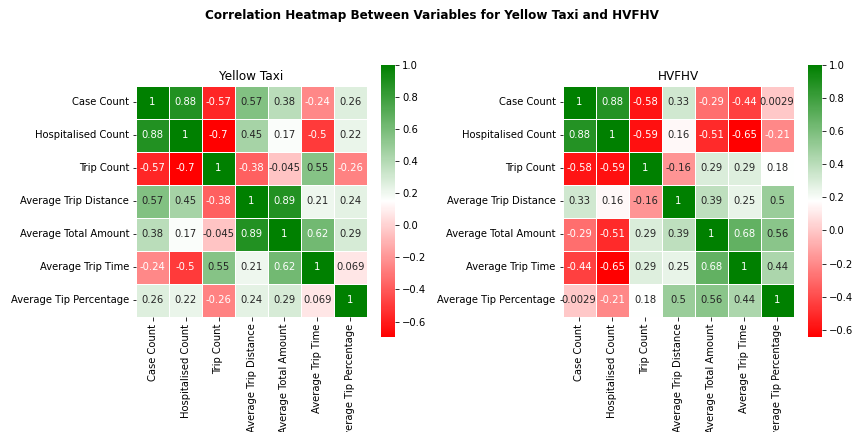
\includegraphics[scale=0.5]{plots/agg_correlation_heatmap.png}
    \caption{Correlation heat map between all selected variables}
\end{figure}

As show in Figure 3, unsurprisingly many features within each data-set such as ``Case Count'' and ``Hospitalised Count'' or ``Average Trip Distance'' and ``Average Total Amount'' are strongly correlated with each other. 

There were however some evidence of correlation between other attributes as listed:
\begin{itemize}
    \item Seems to be a fairly strong negative correlation between ``Hospitalised Count'' and ``Trip Count'' as well as ``Case Count'' and ``Trip Count''. This relationship in both heat-maps have a correlation factor of under -0.5 with the strongest correlation being -0.7 between ``Hospitalised Count'' and ``Trip Count'' of the Yellow Taxi
    \item There seems to be some evidence of correlation between ``Hospitalised Count'' and ``Average Trip Time'' especially in the HVFHV with a correlation of -0.65
    \item A moderate positive correlation is observed between ``Case Count'' and ``Hospitalised Count'' with ``Average Trip Distance'' in the Yellow Taxis of 0.57 and 0.45 respectively
\end{itemize}

While there is some evidence of correlation, this does not necessarily mean a direct causal relationship between the two features. Nevertheless, the relationship between trip counts and COVID-19 statistics are useful in determining how COVID-19 has affected the industry so will be further investigated in the next section.

\subsection{Feature Relationships Analysis Against Time}
In this section, a deeper focus and analysis is performed on the ``Trip Count'' and ``Average Tip Percentage'' features. 

\subsubsection{Trip Count}

\begin{figure}[H]
    \centering
    \begin{subfigure}[b]{0.49\textwidth}
        \centering
        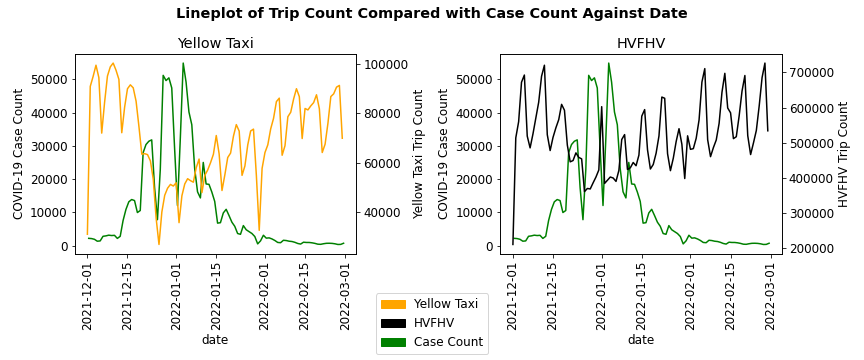
\includegraphics[width=\textwidth]{plots/trip_count_vs_CASE_COUNT_lineplot.png}
        \caption[]%
        {{\small Trip Count vs Case Count}}    
        \label{}
    \end{subfigure}
    \hfill
    \begin{subfigure}[b]{0.49\textwidth}  
        \centering 
        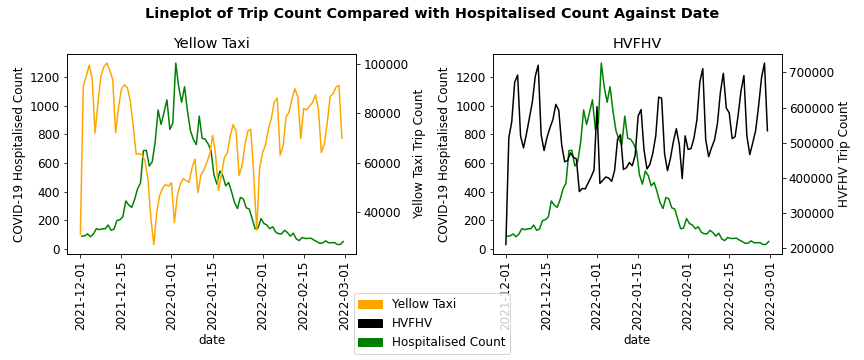
\includegraphics[width=\textwidth]{plots/trip_count_vs_HOSPITALIZED_COUNT_lineplot.png}
        \caption[]%
        {{\small Trip Count vs Hospitalisation Count}}    
    \end{subfigure}
    \vskip\baselineskip
    \caption[]
    {\small Line-plots of trip count of Yellow Taxis and HVFHV compared to COVID-19 case counts and hospitalisation counts} 
\end{figure}

In Figure 4, it is clear that the Yellow Taxi industry was hit with the hardest decrease in trips throughout the 2021-2022 period and there seems to be a correlation between Case Count and Hospitalisation Count for both industries. The more dire impact on Yellow Taxi trip counts could be due to less people willing to go outside and thus less opportunities to hail a Yellow Taxi, however all features could be attributed to the usual holiday season trends i.e. less people travel during Christmas and New Year's, but also more gatherings leading to higher COVID-19 cases.

\subsubsection{Average Tip Percentage}
While average tip percentage did not have significant correlation between any other features in Figure 3, it is a useful indicator of how passengers' behaviour have changed after the pandemic.

\begin{figure}[H]
    \centering
    \begin{subfigure}[b]{0.49\textwidth}
        \centering
        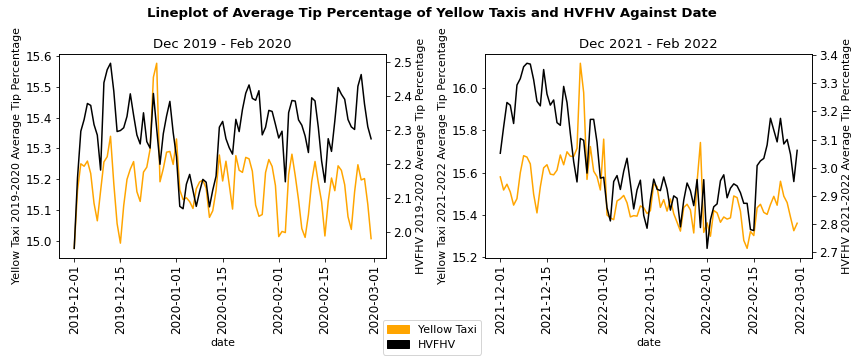
\includegraphics[width=\textwidth]{plots/tip_percent_avg_timeline_lineplot.png}
        \caption[]%
        {{\small Average Tip Percentage vs Date of 2019-2020 and 2021-2022}}    
        \label{}
    \end{subfigure}
    \hfill
    \begin{subfigure}[b]{0.49\textwidth}  
        \centering 
        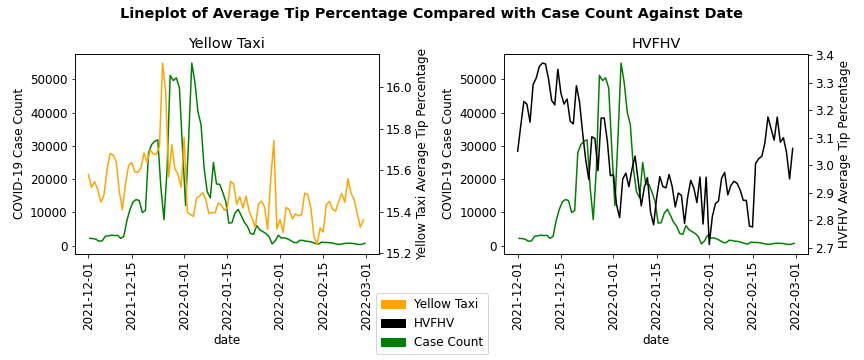
\includegraphics[width=\textwidth]{plots/tip_percent_avg_vs_CASE_COUNT_lineplot.png}
        \caption[]%.
        {{\small Average Tip Percentage vs Case Count of 2021-2022}}    
    \end{subfigure}
    \vskip\baselineskip
    \caption[]
    {\small Line-plots of average tip percentages compared to date} 
\end{figure}

Although in Figure 5b it doesn't seem as though there is any significant relationship between COVID-19 case counts and tipping behaviour, interestingly from Figure 7a it is observed that tip percentage has increased in 2021-2022 compared to 2019-2020, with percentages at its peak in around 2021 December. The generally higher tip amounts throughout December could be attributed to the holiday season, and passengers being more willing and generous in tipping or travelling longer distances. 

\section{Statistical Modelling}
This section builds two Ordinary Least Squares (OLS) Linear Regression models to test COVID-19's direct effect on Trip Counts and tipping behaviour before, and after the pandemic. Both models are evaluated against a baseline model that uses the mean as the predicted value, and are evaluated using the Root Mean Squared Error (RMSE) \cite{rmse} and \(R^2\) value \cite{r_squared}. 

\subsection{Predicting Trip Count Using COVID-19 Data}
This model aims to investigate the existence of a direct relationship between COVID-19 daily Case and Hospitalisation Counts against Trip Counts. The data was split into 80\% training and 20\% testing using random sampling, before an OLS Linear Regression model was trained on the training set and evaluated with the testing set.

\begin{table}[H]
    \centering
    \begin{tabularx}{\linewidth}{|l|l||*{4}{X|}}
        \hline
        \multicolumn{6}{|c|}{Evaluation Metrics for OLS of Trip Count Predictions} \\
        \hline 
        Data-set & Model & \multicolumn{2}{|c|}{Train Data} & \multicolumn{2}{|c|}{Test Data}\\
        \cline{3-6}
        & & RMSE & \(R^2\) & RMSE & \(R^2\)\\
        \hline 
        Yellow Taxi & Baseline &  16378.2763 & 0.0000 & 21596.5521 & -0.0099\\
        & Linear Regression & 11546.7579 & 0.5030 & 15657.1997 & 0.4692 \\
        \hline
        HVFHV & Baseline & 95954.6975 & 2.2204 & 102583.4463 & -0.0174 \\
        & Linear Regression & 78430.1178 & 0.3319 & 75356.0436 &  0.4510 \\
        \hline
    \end{tabularx}
    \caption{Evaluation Metrics for OLS of Trip Count Prediction}
    \label{tab:my_label}
\end{table}

As in Table 1, the model built on Yellow Taxis and HVFHV performed similarly with an \(R^2\) value of 0.4692 and 0.4510 respectively. While both performed better than the baseline, the results do not show an exceptionally high correlation between the COVID-19 features and Trip Counts. Nevertheless, the Yellow Taxi daily trip counts range from approximately 25,000 to 100,000 and HVFHV from approximately 200,000 to 725,000, which when compared to the RMSE (Root Mean Squared Error) in Table 1 shows model performance is not exceptionally low either. 

\subsection{Comparison of Tipping Behaviour Before and After COVID-19}

This model investigates how tipping behaviour has changed before and after the pandemic by attempting to predict daily average trip percentages of 2021-2022 using data from 2019-2022 with an OLS Linear Regression model. The features used for this model were daily trip count, average trip distances, average total amounts, and average trip times. 

\begin{table}[]
    \centering
    \begin{tabularx}{\linewidth}{|l|l||*{4}{X|}}
        \hline
        \multicolumn{6}{|c|}{Evaluation Metrics for OLS of Average Tip Percentage Predictions} \\
        \hline 
        Data-set & Model & \multicolumn{2}{|c|}{Train Data (2019-2020)} & \multicolumn{2}{|c|}{Test Data (2021-2022)}\\
        \cline{3-6}
        & & RMSE & \(R^2\) & RMSE & \(R^2\)\\
        \hline 
        Yellow Taxi & Baseline &  0.1000 & 0.0000 & 0.3434 & -4.7004\\
        & Linear Regression & 0.0807 & 0.3489 & 0.2149 & -1.2319 \\
        \hline
        HVFHV & Baseline & 0.1053 & 0.000 & 0.7463 & -20.5382 \\
        & Linear Regression & 0.0806 & 0.2772 & 0.8843 & -29.2400 \\
        \hline
    \end{tabularx}
    \caption{Evaluation Metrics for OLS of Average Tip Percentage Predictions}
    \label{tab:my_label}
\end{table}

From Table 2, it can be seen that both Yellow Taxi and HVFHV models performed very poorly with \(R^2\) values below 0 indicating the models built are unable to make accurate predictions. In fact, the Linear Regression model of the HVFHV data-sets performed even poorer than the Baseline model. In addition, the large increase in the RMSE of the test data compared to the training data indicates the models were over-fitted and are not a good generalisation. The poor performance may be an indication of a change in tipping behaviour as the 2021-2022 data is unexplainable using the 2019-2022 data 

\subsection{Diagnostics}

Upon examining diagnostic plots, it can be observed that both models do not follow the linear model assumption as there is significant heteroscedacity in the Residuals vs Fitted and Scale-Location plots. Therefore these models may not be entirely suitable for predictions but nevertheless can be used as a guide.

\section{Discussion and Recommendations}
Interesting observations were made in passenger behaviour before and after the pandemic and during its peak in numbers in December 2021 to February 2022. Recommendations can be made from the results of the analysis and modelling for decision makers amongst the Yellow Taxi and HVFHV industries.

Key decision makers in both industries are recommended to use key statistics and forecasting during crises occurring in the USA to aid in modelling and forecasting trip counts and demand during such times. For example, in Figures 3 and 4 there is evidence of correlation between COVID-19 case and hospitalisation counts with daily trip counts. The average performance of Model 1 as shown in Table 1 also indicates that these statistics can be used not as a main tool but an approximate guide in forecasting trip counts during crises. Nevertheless, correlation and this modelling cannot be solely relied on as these features may both be directly correlated with other factors such as holiday seasons.

Another key takeaway from the analysis is that key decision makers should ensure close attention is paid to driver-targeted marketing during expected high traffic periods (such as recovery from a pandemic and holidays) as tips seem to be at its highest during these periods. From Figure 5 it seems that tips are at its highest in December 2021 as NYC celebrates its first holiday season after COVID-19 vaccines being introduced. In addition, while Model 2 had quite a poor performance as observed in Table 2, this may indicate a change in tipping behaviour and thus 2021-2022 is unable to be modelled using 2019-2020 data. Decision makers can use this analysis on tipping in promotional campaigns at specific time periods encouraging more people to drive for their company, or to encourage drivers to get back on the road following a major crisis thus minimising driver shortages. 

\section{Conclusion}
This report aimed to investigate the impact of COVID-19 on the Yellow Taxi and HVFHV industry during the late 2021 spike, and also analyse the change in behaviour of passengers before and after the height of pandemic restrictions and lock-downs. While it is clear that COVID-19 has adversely impacted the industry in daily trip numbers, the data throughout this period can be useful to aid forecasting in future crises of a similar scale. With COVID-19 still lingering on people's minds, it may be of interest to investigate further into how COVID-19 has affected driver behaviours as well.

\clearpage

% BEGIN REFERENCES SECTION
\printbibliography

\end{document}